% !TeX root = ../main.tex
% !TeX encoding = UTF-8
% !TeX spellcheck = none
\subsection{超参数敏感性分析}\label{sec:exp-hyperparameters}

我们在成都数据集上开展单变量验证集敏感性实验，考察SERR门控隐藏维度、BCMS内部表征维度，以及两条残差通路的初始化参数。两个维度均在\(\{8,16,32,64,128\}\)中取值，\(\alpha_0\)与\(\beta_0\)均在\(\{0,0.001,0.01,0.05,0.1\}\)中取值。参考配置沿用主要对比实验的默认值\((32,32,0,0)\)，每次仅改变其中一个参数，其余设置保持不变。

验证指标采用正目标值掩码。在每个验证批次内，将样本、网格和12个预测步中的有效位置合并，分别计算流入与流出的MAE和RMSE；对两通道指标等权平均得到批次联合指标，再对各验证批次等权平均。成都的1,724个验证窗口补齐为1,728个窗口，以27个批次参与计算，4个补齐的重复窗口保留在统计中。本节报告上述批次平均验证误差，与第\ref{sec:exp-baselines-metrics}节测试集AVG12的汇总口径不同。

\begin{figure}[!htbp]
  \centering
  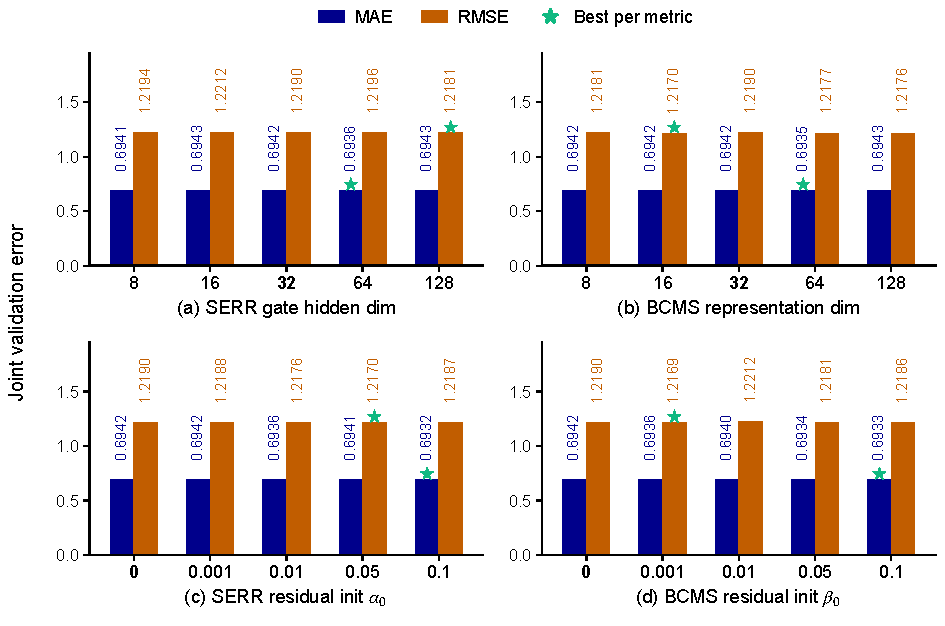
\includegraphics[width=\linewidth]{figures/hyperparameter-joint.pdf}
  \caption[联合验证指标的超参数敏感性]{\textbf{成都数据集上联合验证指标的超参数敏感性。}（a）SERR门控隐藏维度；（b）BCMS内部表征维度；（c）SERR残差强度初值\(\alpha_0\)；（d）BCMS残差参数初值\(\beta_0\)。蓝色和橙色柱分别对应MAE和RMSE，绿色星号标记每组中各指标的最小值，加粗横轴刻度表示参考配置；柱上数值保留四位小数，星号依据未舍入值确定。指标按正文所述验证批次口径汇总，联合指标对流入和流出等权平均。每个配置为固定种子42的一次运行，两项指标均在最低联合验证MAE所选检查点上计算。}
  \label{fig:hyperparameter-joint}
\end{figure}

图~\ref{fig:hyperparameter-joint}展示四组参数对应的联合验证误差。以每组最大与最小误差之差除以参考配置误差，四组联合MAE的相对极差均低于0.15\%，联合RMSE的相对极差均低于0.35\%。因此，在本次扫描范围内，四个参数的调整仅引起较小的验证误差变化。

隐藏维度的增大未带来单调改善。SERR门控隐藏维度为64时取得该组最低联合MAE，而最低联合RMSE出现在128；BCMS表征维度的对应最优值则分别为64和16。不同指标偏好的维度并不一致，较宽的内部表示也未在两项指标上形成持续优势。

残差初值直接赋给可学习参数，即\(\alpha(0)=\alpha_0\)、\(\beta(0)=\beta_0\)，其中BCMS的初始有效系数为\(\tanh(\beta_0)\)；两参数随后均参与训练。\(\alpha_0\)和\(\beta_0\)均在0.1时取得各自组内最低联合MAE，分别为0.693224和0.693278；最低联合RMSE则分别出现在\(\alpha_0=0.05\)和\(\beta_0=0.001\)。这些最小值与零初始化参考配置之间的差异较小，说明本次扫描中的组内最佳取值随评价指标而变化。

图~\ref{fig:hyperparameter-flow}进一步给出流入与流出的分通道结果。以SERR门控为例，流入MAE和RMSE的最优维度分别为64和128，而流出的两项指标均在维度8时最小；BCMS维度64则同时取得流出MAE和RMSE的最小值。这表明联合指标中的小幅变化仍包含通道间的不同响应，超参数比较应同时关注整体误差与分通道表现。



\begin{figure}[!htbp]
  \centering
  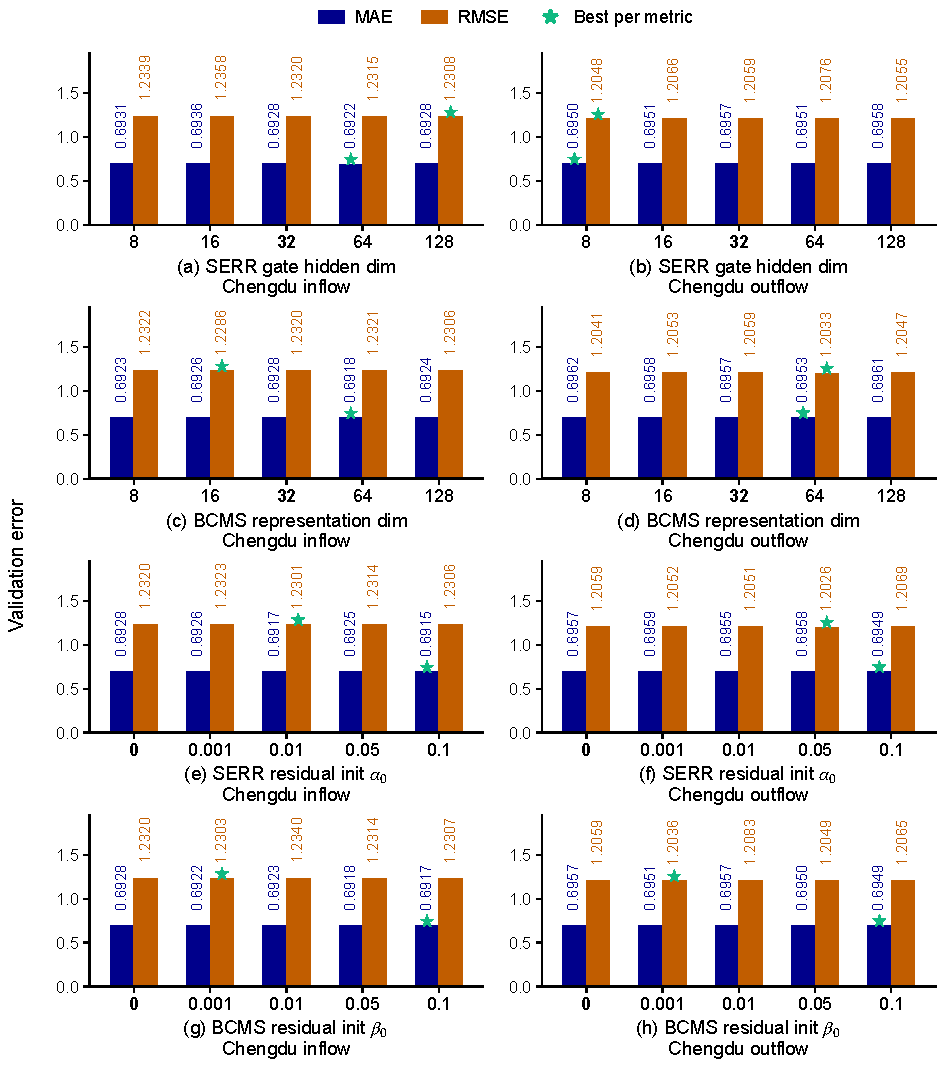
\includegraphics[width=\linewidth]{figures/hyperparameter-flow.pdf}
  \caption[流入与流出的超参数敏感性]{\textbf{成都数据集上流入与流出的超参数敏感性。}左列为流入，右列为流出；四行依次对应SERR门控隐藏维度、BCMS内部表征维度、\(\alpha_0\)和\(\beta_0\)。蓝色和橙色柱分别表示各通道按验证批次等权平均的MAE与RMSE，绿色星号标记组内最小值。参考刻度与数值显示规则同图~\ref{fig:hyperparameter-joint}。}
  \label{fig:hyperparameter-flow}
\end{figure}
